\documentclass[10pt,pdf,hyperref={unicode}]{beamer}


\usepackage[T2A]{fontenc}
\usepackage[utf8x]{inputenc}
\usepackage[english,russian]{babel}

\usepackage{amssymb,amsmath}

\usetheme{Berkeley}
%\useoutertheme{dove}
\usecolortheme{dove}
%\usecolortheme[named=Brown]{structure} 
%\usecolortheme[RGB={205,173,0}]{structure} 


\graphicspath{{images/}}

%\usefonttheme[onlymath]{serif}
\title[\theme]{Синтез математической модели \\
джиттера прибытия пакетов}

\author[Кобрин А. В.]{Кобрин Артем Витальевич}
\institute[ХНУРЭ]{Харьковский Национальный Университет Радиоэлектроники\\
	{\tiny Кафедра ТКС}\\
}
\date{2013}
\begin{document}



% титульная стр
\begin{frame}
\titlepage
\end{frame}
 
\section{Обзор типов джиттера}

\begin{frame}
\frametitle{Обзор типов джиттера}
    \textbf{Выделяют три типа джиттера, которые могут быть вызваны различными причинами}:
    \begin{itemize}
        \item Постоянный джиттер - это стандартная передача пакетов с примерно постоянным изменением задержки.
        \item Джиттер содержащий выбросы задержки возникает, когда один пакет в потоке оказывается задержанным на значительно больший интервал времени по отношению к другим. 
        \item Джиттер содержащий скачкообразное изменения задержки, при котором задержка прибытия пакетов изменяется для целого ряда пакетов в потоке.
    \end{itemize}

\end{frame}

\section{Основные типы джиттера пакетной задержки}

\begin{frame}
\frametitle{Основные типы джиттера пакетной задержки}
\begin{figure} [!h] 
  \center
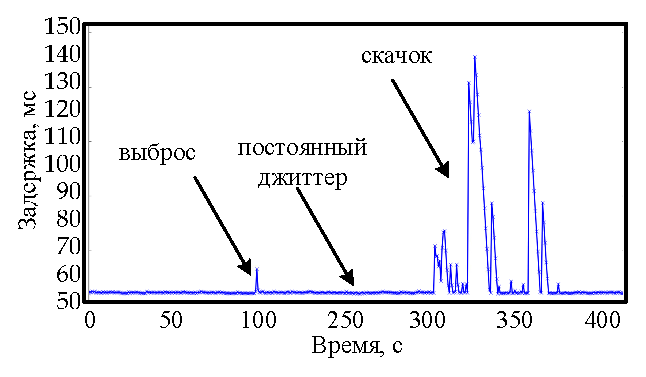
\includegraphics{3typeJitter.eps}

  \label{img:3typeJitter}  
\end{figure}

\end{frame}

\section{Анализ причин джиттера в проводной сети}

\begin{frame}
\frametitle{Название слайда}
    \textbf{Нумерованный список}:
    \begin{itemize}
        \item Раз
        \item Два
        \item Три
    \end{itemize}
\begin{exampleblock}{Пример}
         Текст примера
\end{exampleblock}
\begin{equation}
\B{LoG}(\sigma;x,y) = \nabla^2 \B{G} =
\rev{\sigma^3\sqrt{2\pi}}\Bigl(2-\frac{x^2+y^2}{\sigma^2}\Bigr)
\e^{-\frac{x^2+y^2}{2\sigma^2}}.
\label{log}
\end{equation}
Комбинация фильтров Лапласа и Гаусса и есть оператор лапласиана гауссианы.
\end{frame}


\end{document}